\section{Jismning og`irlik markazi}

\begin{enumerate}

\item Aylanish o‘qidan kuch qo‘yilgan nuqtagacha bo‘lgan masofa 2,5 m, aylanish o‘qidan kuchning ta’sir chizig‘i-gacha bo‘lgan masofa 1,5 m. Agar kuchning kattaligi 50 N bo‘lsa, kuch momentini toping ($N \cdot m$). [2]
\begin{enumerate}[label=\Alph*)]
\item 75
\item 50
\item 100
\item 125
\end{enumerate}

\item Kuchni uch marta orttirib, yelkani 2 marta kamaytirsak, kuch momenti qanday o‘zgaradi? [2]
\begin{enumerate}[label=\Alph*)]
\item 1,5 marta ortadi
\item 1,5 marta kamayadi
\item 3 marta ortadi
\item 3 marta kamayadi
\end{enumerate}

\item Qanday shartlar bajarilganda aylanish o‘qiga ega bo‘lgan jism muvozanatda bo‘ladi? Agar ... [2]
\begin{enumerate}[label=\Alph*)]
\item kuchlarning geometrik yig‘indisi nolga teng bo‘lsa
\item jismni o‘ngga va chapga aylantiruvchi kuchlar momentlarining noldan farqli bo‘lsa
\item musbat va manfiy kuch momentlarining yig‘indisi teng bo‘lsa
\item kuchlarning algebraik yig‘indisi noldan farqli bo‘lsa
\end{enumerate}

\item Aylanish o‘qidan kuch qo‘yilgan nuqtagacha bo‘lgan masofa $d$ bo‘lsa, rasmdan foydalanib kuch momentini toping. [3]

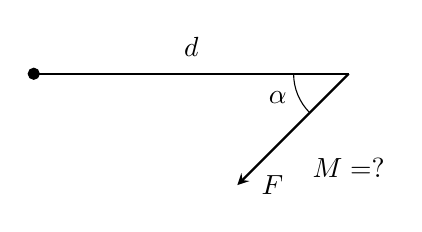
\begin{tikzpicture}[>=stealth, scale=1]
    % Aylanish o'qi (richag)
    \draw[thick] (0,0) -- (4,0);
    
    % Tayanch nuqtasi (bold dot)
    \filldraw (0,0) circle (2pt);
    
    % Masofa belgisi (d)
    \node[above] at (2,0.1) {$d$};
    
    % Kuch vektori (F)
    % Burchak rasmda richag va kuch yo'nalishi orasida ko'rsatilgan
    \draw[->, thick] (4,0) -- ++(225:2) node[right, xshift=5pt] {$F$};
    
    % Burchak yoyi (alpha)
    \draw (3.3,0) arc (180:225:0.7);
    \node at (3.1,-0.3) {$\alpha$};
    
    % So'ralayotgan kattalik (M=?)
    \node at (4,-1.2) {$M=?$};

\end{tikzpicture}

\begin{enumerate}[label=\Alph*)]
\item $M = Fd \cdot tg\alpha$
\item $M = Fd$
\item $M = Fd \cdot \cos\alpha$
\item $M = Fd \cdot \sin\alpha$
\end{enumerate}

\item Richagning kichik yelkasiga 300 N kuch, katta yelkasiga 20 N kuch ta’sir qiladi. Kichik yelkaning uzunligi 5,0 sm. Katta yelkaning uzunligini aniqlang (sm). [4]
\begin{enumerate}[label=\Alph*)]
\item 75
\item 40
\item 150
\item 35
\end{enumerate}

\item Richagning uchlariga 40 N va 240 N kuchlar ta’sir qiladi, tayanch nuqtasidan kichik kuchgacha bo‘lgan oraliq 60 sm. Agar richag muvozanatda bo‘lsa, richagning uzunligini aniqlang (sm). [4]
\begin{enumerate}[label=\Alph*)]
\item 9
\item 14
\item 70
\item 7
\end{enumerate}

\item Uzunligi 1 metr bo‘lgan vaznsiz richag uchlarida 5 kg dan ikkita yuk osilgan. Tayanch yuklarning biridan 20 sm masofada joylashgan. Shu uchidan qanday masofaga 30 kg yuk qo‘yilsa, richag muvozanatda bo‘ladi? (sm) [4]
\begin{enumerate}[label=\Alph*)]
\item 8
\item 12
\item 10
\item 15
\end{enumerate}

\item Richagning umumiy uzunligi 200 sm. Uning bir uchiga osilgan 10 kg massali yuk ikkinchi uchiga osilgan 40 kg massali yuk bilan muvozanatda turishi uchun tayanch ikkinchi uchidan qanday masofada (sm) joylashishi kerak? [4]
\begin{enumerate}[label=\Alph*)]
\item 40
\item 10
\item 50
\item 20
\end{enumerate}

\item Sterjenga qarama-qarshi tomonga yo‘nalgan parallel 10 N va 25 N kuchlar ta’sir qiladi. Agar bu kuchlarning qo‘yilish nuqtalari bir-biridan 1,5 m masofada joylashgan bo‘lsa, bu kuchlarni muvozanatlovchi kuchning kattaligi (N) va qo‘yilish nuqtasini toping (m). [5]
\begin{enumerate}[label=\Alph*)]
\item 15; 2,5
\item 30; 2,5
\item 25; 5
\item To‘g‘ri javob yo‘q
\end{enumerate}

\item Quyidagi qaysi qurilma yordamida $F$ kuch bilan $m$ massali yukni biror $h$ balandlikka ko‘tarishda ishdan yutish mumkin? [5]

\begin{tikzpicture}[>=stealth, scale=0.8]
    % --- 1. Qiya tekislik (chapda) ---
    \begin{scope}[xshift=0cm]
        \draw[thick] (0,0) -- (3,2) -- (3,0) -- cycle;
        \draw[thick, rotate around={33.7:(1.5,1)}] (1,1) rectangle (2,1.6);
        \node at (1.5,1.5) {$m$};
        \draw[->, thick] (1.75,1.55) -- ++(33.7:1.5) node[above] {$F$};
    \end{scope}

    % --- 2. Richag / Egilgan sterjen (markazda) ---
    \begin{scope}[xshift=4.5cm]
        \draw[thick] (0,3) -- (1.5,1.5) -- (1.5,0.5);
        \filldraw (1.5,1.5) circle (2pt);
        \draw[thick] (1.2,0) rectangle (1.8,0.5);
        \node at (1.5,0.25) {$m$};
        \draw[->, thick] (0,3) -- (0,2) node[left] {$F$};
    \end{scope}

    % --- 3. Qo'zg'almas blok (o'ngda) ---
    \begin{scope}[xshift=8.5cm]
        % Shift (Ceiling)
        \fill[pattern=north east lines] (-1,3.2) rectangle (1,3.4);
        \draw[thick] (-1,3.2) -- (1,3.2);
        
        % Blok tayanchi
        \draw[thick] (0,3.2) -- (0,2.5);
        \draw[thick] (0,2) circle (0.5);
        \filldraw (0,2) circle (1.5pt);
        
        % Iplar va yuk
        \draw[thick] (-0.5,2) -- (-0.5,1); % Chap ip
        \draw[->, thick] (-0.5,1) -- (-0.5,0.5) node[left] {$F$};
        
        \draw[thick] (0.5,2) -- (0.5,1); % O'ng ip
        \draw[thick] (0.2,0.4) rectangle (0.8,1);
        \node at (0.5,0.7) {$m$};
    \end{scope}
\end{tikzpicture}

\begin{enumerate}[label=\Alph*)]
\item qo‘zg‘almas blok yordamida
\item richag yordamida
\item qiya tekislik yordamida
\item uchovida teng ish bajariladi
\end{enumerate}

\item Rasmda vaznsiz richagga osilgan 3 kg va 2 kg massali jismlar muvozanatlashgan. Agar richagning kuch yelkasi $AB = 30$ cm bo‘lsa, o‘ng yelkasi $BC$ nimaga (cm) teng? [6]

\begin{tikzpicture}[>=stealth, scale=1]
    % Shift (Ceiling) tasviri
    \fill[pattern=north east lines] (-0.6, 1.2) rectangle (0.6, 1.4);
    \draw[thick] (-0.6, 1.2) -- (0.6, 1.2);
    
    % Markazdagi tayanch ipi (C nuqtaga)
    \draw[thick] (0, 1.2) -- (0, 0);
    
    % Richag (ACB sterjeni)
    % AC = 2 birlik, BC = 3 birlik (3kg * 2 = 2kg * 3 muvozanat sharti uchun)
    \draw[thick] (-2, 0) -- (3, 0);
    
    % Nuqtalar va ularning nomlari
    \filldraw (-2,0) circle (1.5pt) node[above left] {A};
    \filldraw (0,0) circle (1.5pt) node[below left] {C};
    \filldraw (3,0) circle (1.5pt) node[above right] {B};
    
    % Chapdagi yuk (3 kg)
    \draw[thick] (-2, 0) -- (-2, -0.6);
    \draw[thick] (-2.4, -0.6) rectangle (-1.6, -1.4);
    \node[right] at (-1.6, -1.0) {3 kg};
    
    % O'ngdagi yuk (2 kg)
    \draw[thick] (3, 0) -- (3, -0.6);
    \draw[thick] (2.7, -0.6) rectangle (3.3, -1.1);
    \node[left] at (2.7, -0.85) {2 kg};

\end{tikzpicture}

\begin{enumerate}[label=\Alph*)]
\item 24
\item 18
\item 15
\item 20
\end{enumerate}

\item Aylanish o‘qi A nuqtada natijaviy kuch momenti 0 ga teng bo‘lsa, $x$ ni toping.

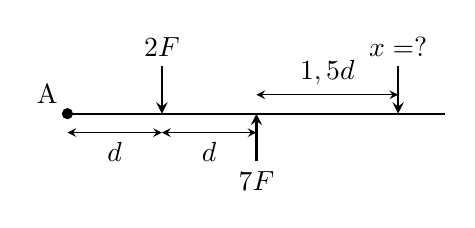
\begin{tikzpicture}[>=stealth, scale=1.2]
    % Sterjen (Gorizontal chiziq)
    \draw[thick] (0,0) -- (4,0);
    
    % A nuqta (Aylanish o'qi)
    \filldraw (0,0) circle (1.5pt) node[above left] {A};
    
    % Birinchi kuch (2F pastga)
    \draw[->, thick] (1, 0.5) -- (1,0) node[pos=0, above] {$2F$};
    
    % Ikkinchi kuch (7F yuqoriga)
    \draw[->, thick] (2, -0.5) -- (2,0) node[pos=0, below] {$7F$};
    
    % Uchinchi kuch (x=? pastga)
    \draw[->, thick] (3.5, 0.5) -- (3.5,0) node[pos=0, above] {$x=?$};
    
    % Masofalar va ularning belgilari
    % A dan 2F gacha masofa d
    \draw[<->, thin] (0, -0.2) -- (1, -0.2) node[midway, below] {$d$};
    
    % 2F dan 7F gacha masofa d
    \draw[<->, thin] (1, -0.2) -- (2, -0.2) node[midway, below] {$d$};
    
    % 7F dan x gacha masofa 1,5d
    \draw[<->, thin] (2, 0.2) -- (3.5, 0.2) node[midway, above] {$1,5d$};

\end{tikzpicture}

\begin{enumerate}[label=\Alph*)]
\item $30F/11$
\item $4F$
\item $28F/7$
\item $24F/7$
\end{enumerate}

\item $OA$ vaznsiz sterjen tayanchga o‘rnatilgan $O$ o‘qqa nisbatan vertikal tekislikda erkin aylana oladi. Sterjenning $A$ uchiga $30^\circ$ burchak ostida 200 N kuch ta’sir etmoqda. Sterjenni muvozanatda saqlash uchun uning o‘rtasidagi $B$ nuqtaga qanday $m$ yuk (kg) qo‘yish kerak?

\begin{tikzpicture}[>=stealth, scale=1.2]
    % Sterjenning asosi (to'rtburchak ko'rinishida)
    \draw[thick] (0,0) rectangle (4,0.15);
    
    % Shartli ravishda sterjenning bo'lingan qismlarini shtrixlash (rasmdagidek)
    \fill[pattern=north east lines] (0,0) rectangle (1,0.15);
    \fill[pattern=north east lines] (2,0) rectangle (3,0.15);

    % O nuqta - Aylanish o'qi (tayanch)
    \draw (0,0) -- (-0.15,-0.25) -- (0.15,-0.25) -- cycle;
    \foreach \x in {-0.15,-0.05,0.05}
        \draw (\x,-0.25) -- (\x+0.05,-0.32);
    \node[above left] at (0,0.15) {O};

    % B nuqta (o'rtada) va osilgan m yuk
    \node[above] at (2,0.15) {B};
    \draw[thick] (2,0) -- (2,-0.4);
    \draw[thick] (1.85,-0.4) rectangle (2.15,-0.75);
    \node at (2,-0.57) {$m$};

    % A nuqta (o'ng chet) va F kuch vektori
    \node[below] at (4,0) {A};
    \draw[->, thick] (4,0.1) --(3,1) node[right] {$F$};
    
    % Alpha burchagi
    \draw (3.47, 0.15) arc (0:-35:-0.6);
    \node at (3.35, 0.3) {$\alpha$};

\end{tikzpicture}

\begin{enumerate}[label=\Alph*)]
\item 25
\item 30
\item 20
\item 43
\end{enumerate}

\item Bir jinsli balka $O$ nuqtaning atrofida aylanishi mumkin. $F_2$ kuch balkaning o‘rtasiga qo‘yilganligi va balkaning muvozanatda ekanligi ma’lum bo‘lsa, kuchlar orasidagi to‘g‘ri munosabatni toping.

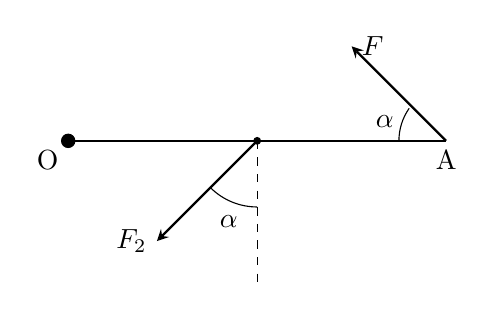
\begin{tikzpicture}[>=stealth, scale=1.2]
    % Balka (Gorizontal sterjen)
    \draw[thick] (0,0) -- (4,0);
    
    % O nuqta - Aylanish o'qi
    \filldraw (0,0) circle (2pt) node[below left] {O};
    
    % Midpoint (F2 qo'yilgan nuqta)
    \filldraw (2,0) circle (1pt);
    
    \node[below] at (4,0) {A};
    \draw[->, thick] (4,0) --(3,1) node[right] {$F$};
    \draw (3.5, 0) arc (0:-35:-0.6);
    \node at (3.35, 0.2) {$\alpha$};
    
    % F2 kuch (o'rtada)
    % Vertikal yordamchi chiziq (punktir)
    \draw[dashed] (2,0) -- (2,-1.5);
    % F2 vektori
    \draw[->, thick] (2,0) -- ++(225:1.5) node[left] {$F_2$};
    % F2 burchagi alpha (vertikalga nisbatan)
    \draw (2,-0.7) arc (-90:-135:0.7);
    \node at (1.7,-0.85) {$\alpha$};

\end{tikzpicture}

\begin{enumerate}[label=\Alph*)]
\item $F_1 = F_2$
\item $F_1 = \sin\alpha \cdot F_2$
\item $F_2 = 2tg\alpha \cdot F_1$
\item $F_1 = 2ctg\alpha \cdot F_2$
\end{enumerate}

\item Massasi 20 kg bo‘lgan bir jinsli kub $O$ nuqtada poldagi qirraga tiralgan. Kubning $B$ chetini bir oz ko‘tarish uchun $A$ nuqtaga qanday gorizontal $F$ kuch qo‘yish kerak (N)?

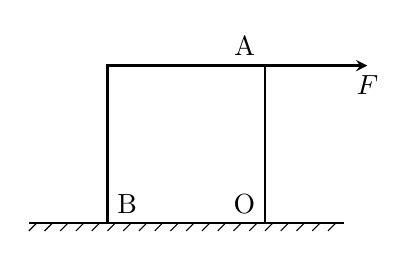
\begin{tikzpicture}[>=stealth, scale=1]
    % Yer (poldagi sirt) tasviri
    \draw[thick] (0.5,0) -- (4.5,0);
    \foreach \x in {0.6,0.8,...,4.4}
        \draw (\x,0) -- (\x-0.1,-0.1);

    % Kubning 2D ko'rinishi (kvadrat)
    \draw[thick] (1.5,0) rectangle (3.5,2);
    
    % Nuqtalarni belgilash (manbadagi rasmga ko'ra)
    \node[above right] at (1.5,0) {B}; % Chap pastki burchak
    \node[above left] at (3.5,0) {O};  % O'ng pastki burchak (tayanch nuqtasi)
    \node[above left] at (3.5,2) {A};  % O'ng yuqori burchak
    
    % F kuch vektori (A nuqtadan o'ngga yo'nalgan)
    \draw[->, thick] (3.5,2) -- (4.8,2) node[below] {$F$};

\end{tikzpicture}

\begin{enumerate}[label=\Alph*)]
\item 10
\item 20
\item 50
\item 100
\end{enumerate}

\item Stolda massasi $m$ uzunligi $l$ bo‘lgan sterjen yotibdi. Bunda uning to‘rtdan bir qismi stoldan chiqib turibdi. Sterjenning shu qismining uchi qanday eng kichik kuch bilan bosilganda, uning boshqa uchi ko‘tarila boshlaydi? 
\begin{enumerate}[label=\Alph*)]
\item $2mg$
\item $mg/2$
\item $mg$
\item $mg/3$
\end{enumerate}

\item Og‘irligi 24 kN bo‘lgan avtomobilning og‘irlik markazidan o‘tkazilgan vertikal avtomobil o‘qlari orasidagi masofani 1:3 nisbatda bo‘lsa, har bir juft g‘ildirakning yo‘lga bo‘lgan bosim kuchlarini toping (kN).
\begin{enumerate}[label=\Alph*)]
\item 6; 6
\item 9; 6
\item 18; 6
\item 18; 12
\end{enumerate}

\item Uzunligi $L$ bo‘lgan silindrsimon sterjenning yarmi $\rho$, yarmi esa $\frac{1}{3}\rho$ zichlikka ega bo‘lgan metaldan tayyorlangan bo‘lsa, uning og‘irlik markazi sterjen markazidan qancha masofada joylashgan?
\begin{enumerate}[label=\Alph*)]
\item $L/16$
\item $L/20$
\item $L/8$
\item $L/4$
\end{enumerate}

\item Bir jinsli, ishqalanishsiz harakatlanadigan, uzunligi 2 m, massasi 100 kg bo‘lgan aravachaning ikki chetida massalari mos holda 70 kg va 90 kg bo‘lgan ikkita bola turibdi. Birinchi bola aravachaning o‘rtasigacha kelganda sistema og‘irlik markazi qanchaga (m) siljiydi?
\begin{enumerate}[label=\Alph*)]
\item 0,27
\item 0,13
\item 0,42
\item 0
\end{enumerate}

\item Massalari 1kg, 5 kg, 7 kg, 3 kg bo‘lgan to‘rtta bir jinsli shar vaznsiz sterjenga shunday mahkamlanganki, ularning markazlari bir-biridan teng masofada ($d = 0,2$ m) yotadi. Sistemaning og‘irlik markazi uchinchi shar markazidan qanday masofada joylashgan (m)?
\begin{enumerate}[label=\Alph*)]
\item -1,5
\item -0,5
\item -0,2
\item -0,05
\end{enumerate}

\item Ikki tomoni alyuminiy uchinchisi mis simdan qilingan teng tomonli uchburchak shakliga ega bo‘lgan ramkaning og‘irlik markazi mis simdan qanday masofada joylashgan (sm)? [9]
\begin{enumerate}[label=\Alph*)]
\item 32,6
\item 14
\item 1,12
\item 10
\end{enumerate}

\item Bir jinsli sterjen 1/3 qismi stol chetidan chiqqan holda muvozanatda turibdi. Bunda stol tomonidagi uchiga 50 N kuch qo‘yilgan bo‘lsa, sterjenning massasini aniqlang (kg). [10]
\begin{enumerate}[label=\Alph*)]
\item 10
\item 14
\item 12
\item 20
\end{enumerate}

\item 30 kg va 40 kg massali jismlar 30 kg massali balkaning chetlarida turibdi. Balkaning uzunligi 4 m ga teng. Balkaning tayanch nuqtasi birinchi jismdan qanday masofada (m) joylashgan? [10]
\begin{enumerate}[label=\Alph*)]
\item 1,8
\item 3,2
\item 2,8
\item 2,2
\end{enumerate}

\item Bir uchiga 120 N yuk osilgan sterjenga yukdan sterjen uzunligining 1/5 qismiga teng masofada tirgovich qo‘yilsa, u gorizontal holatda muvozanatda bo‘ladi. Sterjenning og‘irligi qancha (N)? [10]
\begin{enumerate}[label=\Alph*)]
\item 80
\item 60
\item 40
\item 100
\end{enumerate}

\item Massasi 200 kg va uzunligi 5 m bo‘lgan to‘singa uchlarining biridan 3 m masofada 250 kg massali yuk osilgan. To‘sinning uchlariga tayanchlar qo‘yilgan. Har qaysi tayanchga ta’sir etadigan bosim kuchi qanday (kN)? [10]
\begin{enumerate}[label=\Alph*)]
\item 2,5; 4
\item 5; 2
\item 4; 2
\item 2,5; 2
\end{enumerate}

\item Massasi 100 kg bo‘lgan bir jinsli balka $A$ va $B$ tayanchlarda yotibdi. $A$ tayanchdan $l/4$ masofada massasi 80 kg bo‘lgan yuk bor. Balkaning tayanchlarga beradigan bosim kuchlarini (N) toping. $g=10 m/s^2$.

\begin{tikzpicture}[>=stealth, scale=1.2]
    % Zamin (Ground) chiziqlari tayanchlar ostida
    \draw[thick] (-0.4,-0.5) -- (0.4,-0.5);
    \foreach \x in {-0.3,-0.1,0.1,0.3}
        \draw (\x,-0.5) -- (\x-0.1,-0.6);

    \draw[thick] (3.6,-0.5) -- (4.4,-0.5);
    \foreach \x in {3.7,3.9,4.1,4.3}
        \draw (\x,-0.5) -- (\x-0.1,-0.6);

    % Tayanchlar (Uchburchak ko'rinishida)
    \draw[thick] (0,0) -- (-0.3,-0.5) -- (0.3,-0.5) -- cycle;
    \draw[thick] (4,0) -- (3.7,-0.5) -- (4.3,-0.5) -- cycle;

    % Bir jinsli balka (Shtrixlangan to'rtburchak)
    \draw[thick, pattern=north east lines] (0,0) rectangle (4,0.3);
    
    % Yuk (m) - A tayanchdan taxminan l/4 masofada
    \draw[thick, fill=white] (0.7, 0.3) rectangle (1.3, 0.7);
    \node at (1, 0.5) {$m$};
    
    % Balkaning og'irlik markazidan yo'nalgan mg kuchi
    \filldraw (2, 0.15) circle (1.2pt);
    \draw[->, thick] (2, 0.15) -- (2, -0.6) node[right] {$mg$};

\end{tikzpicture}

\begin{enumerate}[label=\Alph*)]
\item 1300; 500
\item 1200; 600
\item 1100; 700
\item 1050; 750
\end{enumerate}

\item 40 kg massali balka ustiga 10 kg massali yuk qo‘yilgan (rasmga ko‘ra). Chap tayanchda qanday reaksiya kuchi (N) hosil bo‘ladi?

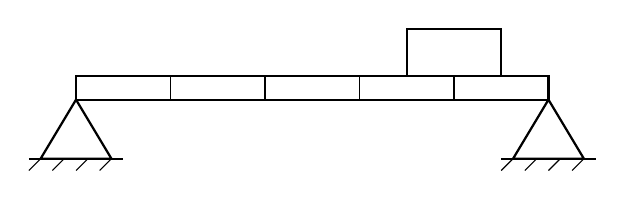
\begin{tikzpicture}[>=stealth, scale=1.5]
    % Chap tayanch ostidagi zamin
    \draw[thick] (-0.4,-0.5) -- (0.4,-0.5);
    \foreach \x in {-0.3,-0.1,0.1,0.3}
        \draw (\x,-0.5) -- (\x-0.1,-0.6);

    % O'ng tayanch ostidagi zamin
    \draw[thick] (3.6,-0.5) -- (4.4,-0.5);
    \foreach \x in {3.7,3.9,4.1,4.3}
        \draw (\x,-0.5) -- (\x-0.1,-0.6);

    % Tayanchlar (uchburchaklar)
    \draw[thick] (0,0) -- (-0.3,-0.5) -- (0.3,-0.5) -- cycle;
    \draw[thick] (4,0) -- (3.7,-0.5) -- (4.3,-0.5) -- cycle;

    % Balka (beshta qismga bo'lingan)
    \draw[thick] (0,0) rectangle (4,0.2);
    \foreach \x in {0.8, 1.6, 2.4, 3.2}
        \draw (\x,0) -- (\x,0.2);

    % Yuk (to'rtburchak blok)
    % Rasmga ko'ra yuk 4-bo'linma ustida joylashgan
    \draw[thick] (2.8, 0.2) rectangle (3.6, 0.6);

\end{tikzpicture}

\begin{enumerate}[label=\Alph*)]
\item 200
\item 240
\item 280
\item 300
\end{enumerate}

\item Vintli press rezbasining qadam balandligi 5 mm ga teng. Vintning ust qismiga uzunligi 40 sm bo‘lgan dasta o‘rnatilgan. Press $10^4$ N kuch bilan ta’sir qilish uchun dastaga qanday kuch qo‘yish lozim.
\begin{enumerate}[label=\Alph*)]
\item 125
\item 250
\item 20
\item 400
\end{enumerate}

\item Radiusi $R$ va balandligi $h$ bo‘lgan silindr turgan qiya tekislikning qiyalik burchagi asta-sekin oshirilib borganda, silindr sirpanishi yoki yiqilishi mumkin. Bu ikkala hodisa bir paytda yuz berishi uchun ishqalanish koeffitsienti qanday bo‘lishi kerak?
\begin{enumerate}[label=\Alph*)]
\item $h/R$
\item $R/h$
\item $2R/h$
\item $h/2R$
\end{enumerate}

\item Silindr uzunligi 50 sm bo‘lgan taxtada turibdi. Silindr ag‘anab tushmasligi uchun taxtaning uchlaridan birini qanday eng katta balandlikka (sm) ko‘tarish mumkin?
\begin{enumerate}[label=\Alph*)]
\item 15
\item 8
\item 9,5
\item 12
\end{enumerate}

\item Bir jinsli silindr gorizont bilan $\alpha$ burchak hosil qiluvchi qiya tekislikka qo‘yildi. Agar silindrning balandligi uning radiusidan ikki marta katta bo‘lsa, tekislikning qanday maksimal qiyalik burchagida silindr to‘ntarilib ketmaydi?
\begin{enumerate}[label=\Alph*)]
\item $15^\circ$
\item $90^\circ$
\item $60^\circ$
\item $45^\circ$
\end{enumerate}

\item Silindr uzunligi 82 sm bo‘lgan taxtada turibdi. Silindr ag‘anab tushmasligi uchun taxtani uchlaridan birini qanday eng katta balandlikka (sm) ko‘tarish mumkin? 
\begin{enumerate}[label=\Alph*)]
\item 19,89
\item 14,5
\item 9,95
\item 11,55
\end{enumerate}

\item Silliq vertikal devorga uzunligi 4 sm bo‘lgan arqon bilan 300 g massali shar osilgan. Agar sharning radiusi 2,5 sm bo‘lsa, uning devorga bosim kuchini toping (N).
\begin{enumerate}[label=\Alph*)]
\item 2,56
\item 0,87
\item 1,94
\item 1,23
\end{enumerate}

\item Massasi $m$ bo‘lgan muntazam uchburchak shaklidagi yassi jism qanday $F$ kuch ta’sirida $O$ nuqta atrofida o‘zini aylantirishi mumkin? $\cos 55^\circ \approx 0,5736$.

\begin{tikzpicture}[>=stealth, scale=1.2]
    % Yer (Ground) sirti
    \draw[thick] (0,0) -- (4,0);
    \fill[pattern=north east lines] (0,-0.2) rectangle (4,0);
    
    % Muntazam uchburchak (Regular triangle)
    % Tomoni 2 birlik, balandligi sqrt(3)
    \draw[thick] (1,0) -- (3,0) -- (2, 1.732) -- cycle;
    
    % O nuqta - Aylanish o'qi (chap burchakda)
    \filldraw (1,0) circle (1.5pt) node[above left] {O};
    
    % F kuch vektori (yuqori uchidan chapga yo'nalgan)
    \draw[->, thick] (2, 1.732) -- (0.8, 1.732) node[above] {F};
    
    % 55 graduslik burchak yoyi
    % Kuch yo'nalishi (gorizontal) va uchburchak tomoni orasida
    \draw (1.6, 1.732) arc (180:240:0.4); 
    \node at (1.4, 1.45) {$55^\circ$};

\end{tikzpicture}

\begin{enumerate}[label=\Alph*)]
\item 0,6104 mg
\item 1/2 mg
\item 0,5774 mg
\item 0,866 mg
\end{enumerate}

\end{enumerate}





\begin{table}[h!]
\centering
\caption{STATIKA: To‘g‘ri javoblar jadvali}
\begin{tabular}{|l|c|l|c|l|c|l|c|l|c|}
\hline
\textbf{№} & \textbf{J.} & \textbf{№} & \textbf{J.} & \textbf{№} & \textbf{J.} & \textbf{№} & \textbf{J.} & \textbf{№} & \textbf{J.} \\ \hline
\textbf{3}  & A & \textbf{11} & C & \textbf{21} & B & \textbf{31} & C & \textbf{76} & A \\ \hline
\textbf{4}  & A & \textbf{12} & C & \textbf{22} & D & \textbf{53} & C & \textbf{77} & D \\ \hline
\textbf{5}  & C & \textbf{13} & A & \textbf{24} & C & \textbf{54} & A & \textbf{84} & C \\ \hline
\textbf{6}  & D & \textbf{16} & D & \textbf{25} & C & \textbf{55} & D & \textbf{85} & C \\ \hline
\textbf{10} & A & \textbf{17} & B & \textbf{29} & D & \textbf{56} & D & \textbf{89} & C \\ \hline
\textbf{90} & B & \textbf{91} & D & \textbf{92} & A & \textbf{93} & D & \textbf{94} & D \\ \hline
\textbf{103} & A & \textbf{104} & A & \textbf{74} & D & \textbf{75} & D & \textbf{30} & C \\ \hline
\end{tabular}
\end{table}